% Importé depuis Chapitre.docx (partie 2)
\PFEChapterOpening{Fondation \& Initiation}

\section{Introduction}

Ce chapitre présente la \textbf{conception} et l’\textbf{architecture} de la plateforme CSR : \textbf{exigences fonctionnelles et non fonctionnelles}, \textbf{gestion de projet Scrum} (\emph{product backlog}, sprints et chronologie), schémas \textbf{UML}\footnote{UML : \emph{Unified Modeling Language} (langage de modélisation unifié). Il s’agit d’un ensemble de notations graphiques standardisées pour représenter, analyser et concevoir des systèmes logiciels orientés objet (cas d’utilisation, classes, séquences, etc.).} (cas d’utilisation, diagramme de classes), puis \textbf{choix technologiques} et \textbf{environnements} matériel et logiciel de développement.

\section{Spécification des exigences}

\subsection{Exigences fonctionnelles}

Les exigences fonctionnelles suivantes spécifient les fonctionnalités que le système doit fournir :

\textbf{Gestion des utilisateurs et des sites}

\begin{itemize}
  \item Assurer l’authentification des utilisateurs via un mécanisme sécurisé.
  \item Émettre des jetons d’accès (JWT) et gérer les sessions (rafraîchissement des jetons).
  \item Gérer des profils utilisateurs distincts (Utilisateur Site, Utilisateur Corporate).
  \item Restreindre l’accès aux données en fonction du rôle de l’utilisateur et du site associé.
  \item Permettre au niveau corporate de créer, modifier, désactiver et affecter des utilisateurs aux différents sites.
  \item Gérer les sites et les catégories d’activités CSR.
\end{itemize}

\textbf{Gestion du plan annuel CSR}

\begin{itemize}
  \item Créer des plans annuels CSR (un plan par couple site/année) avec gestion des statuts (brouillon, soumis, validé, rejeté, etc.).
  \item Prendre en charge les modes de validation 101 et 111 (chaîne de validation adaptée aux processus groupe/site).
  \item Ajouter et modifier des activités planifiées rattachées au plan (catégorie, budget prévisionnel, responsable, dates, partenaire externe, impact cible, etc.).
  \item Intégrer la gestion des activités hors plan lorsque le modèle le prévoit.
  \item Gérer le cycle de vie du plan (modification, soumission, validation, rejet, verrouillage).
  \item Autoriser la modification tant que le plan est en état modifiable (brouillon ou période de déverrouillage).
  \item Permettre la soumission du plan pour validation.
  \item Assurer l’approbation ou le rejet par les acteurs corporate, avec validation multi-niveaux si nécessaire.
  \item Verrouiller le plan après validation définitive ou en dehors de la fenêtre de modification.
  \item Importer des fichiers Excel consolidés avec prévisualisation, contrôles (région/pays/site), détection de conflits et paramétrage par plan.
\end{itemize}

\textbf{Gestion des activités CSR réalisées}

\begin{itemize}
  \item Enregistrer la réalisation des activités planifiées.
  \item Ajouter des activités hors plan.
  \item Autoriser la modification des activités tant qu’elles ne sont pas validées.
  \item Soumettre les activités pour validation corporate.
\end{itemize}

\textbf{Comparaison Planifié vs Réalisé}

\begin{itemize}
  \item Comparer automatiquement les budgets prévisionnels et les budgets réels.
  \item Calculer le taux de réalisation des activités.
  \item Identifier les écarts budgétaires.
  \item Mettre en évidence les activités en dépassement de budget.
\end{itemize}

\textbf{Gestion des demandes de modification}

\begin{itemize}
  \item Permettre la soumission de demandes de modification pour les plans ou activités verrouillés (avec justification et pièces jointes).
  \item Permettre aux acteurs corporate de consulter, approuver ou rejeter les demandes.
  \item Définir une durée de déverrouillage lorsque le processus l’exige.
  \item Gérer les documents associés aux demandes ou aux entités métier (plans, activités).
\end{itemize}

\textbf{Gestion des tableaux de bord}

\begin{itemize}
  \item Visualiser les données CSR sous forme de tableaux de bord interactifs.
  \item Afficher les indicateurs clés de performance (KPI) liés aux activités CSR.
  \item Suivre et comparer les budgets planifiés et réalisés.
  \item Analyser l’impact des activités CSR (global et par participant).
  \item Filtrer les données par site, période, catégorie et type d’activité.
  \item Comparer les performances entre sites et régions.
  \item Suivre l’évolution des indicateurs dans le temps.
  \item Distinguer les activités planifiées et hors plan.
  \item Restreindre l’accès aux tableaux de bord selon le rôle utilisateur (Corporate / Site).
  \item Assurer la mise à jour automatique des données à partir de l’entrepôt de données.
\end{itemize}

\textbf{Fonctionnalités transverses}
\begin{itemize}
  \item Gérer le dépôt et la consultation des documents liés aux sites ou aux entités métier.
  \item Notifier les utilisateurs (validation, rejet, rappels, etc.).
  \item Enregistrer les actions significatives dans un journal d’audit.
  \item Assurer l’internationalisation de l’interface (français et anglais) avec gestion des préférences utilisateur.
  \item Permettre la consultation et la mise à jour du profil utilisateur (informations personnelles et préférences de notification).
\end{itemize}

\subsection{Exigences non fonctionnelles}

Afin d’assurer le bon fonctionnement du système, les exigences non fonctionnelles suivantes doivent être respectées :

\textbf{Sécurité}

\begin{itemize}
  \item Protéger les données d’authentification (hachage des mots de passe, absence de stockage en clair).
  \item Authentifier les utilisateurs par jetons et contrôler systématiquement les requêtes API.
  \item Séparer les droits d’accès (Corporate vs Site) et limiter l’accès aux données autorisées.
  \item Protéger les données sensibles (plans, budgets, indicateurs) conformément aux bonnes pratiques (HTTPS, configuration sécurisée du serveur et de la base).
\end{itemize}

\textbf{Fiabilité}

\begin{itemize}
  \item Garantir la cohérence des règles métier (statuts, validations, verrouillages).
  \item Gérer les erreurs côté API et fournir des retours explicites côté interface utilisateur.
  \item Assurer la persistance des données dans une base MySQL avec contraintes d’intégrité.
\end{itemize}

\textbf{Performance}

\begin{itemize}
  \item Garantir des temps de réponse acceptables pour les usages courants (consultation, tableaux de bord, import de fichiers volumineux).
  \item Assurer la montée en charge via une architecture client/serveur (Angular + API Flask).
\end{itemize}
\newpage
\textbf{Traçabilité}

\begin{itemize}
  \item Enregistrer les opérations importantes dans un journal d’audit (création, modification, validation, suppression, etc.).
  \item Conserver l’historique des validations et des demandes de modification.
  \item Assurer l’horodatage et l’identification des acteurs.
\end{itemize}

\textbf{Ergonomie et maintenabilité}

\begin{itemize}
  \item Proposer une interface web responsive avec une navigation structurée par modules.
  \item Organiser le code en modules fonctionnels côté backend (Flask) et frontend (Angular) pour faciliter la maintenance et l’évolution.
\end{itemize}

\subsection{Identification des Acteurs}

Les principaux acteurs du système sont :

\begin{description}
  \item[Utilisateur Corporate] Cet acteur dispose de tous les droits d'accès lui permettant d'administrer l'ensemble de la plateforme CSR. Il gère les comptes utilisateurs et configure les sites et leurs paramètres. Il valide les plans et activités soumis par les sites, traite les demandes de modification des périodes clôturées et analyse les performances consolidées de tous les sites à travers les tableaux de bord et les dashboards Power BI.
  \item[Utilisateur Site] Cet acteur est soit un responsable CSR soit un collaborateur désigné au sein d'un site géographique de l'entreprise. Il dispose de droits d'accès limités à son propre site, ce qui lui permet d'assurer la gestion opérationnelle des activités CSR qui lui sont rattachées. Il crée et soumet le plan annuel CSR, déclare les activités réalisées planifiées ou hors plan, renseigne les données de réalisation et suit l'avancement de son budget et de ses KPIs. En cas de besoin, il soumet des demandes de modification pour les périodes clôturées et apporte les corrections suite à un rejet.
\end{description}

\subsection{Diagramme de cas d’utilisation générale}

La figure 2.1 présente le diagramme de cas d’utilisation général, décrivant les interactions entre les acteurs et les fonctionnalités du système.

\begin{figure}[H]
  \centering
  \includegraphics[width=0.9\linewidth]{figures/chapitre-02/diagramme_de_cas_utilisation_global.png}
  \caption{Diagramme de cas d’utilisation général.}
  \label{fig:doc-ch2-1}
\end{figure}

\section{Le pilotage du projet par SCRUM}

\subsection{Product Backlog}

Le \emph{product backlog} est une liste dynamique des fonctionnalités qui définissent le périmètre du projet. Il regroupe des \textbf{user stories}, c’est-à-dire des descriptions de besoins du point de vue de l’utilisateur final, généralement structurées selon le schéma suivant : 
 
\vspace{0.8em}
« En tant que \emph{[utilisateur]}, je veux \emph{[réaliser une action]} afin de \emph{[atteindre un objectif]}. »
\vspace{0.8em}

Cette distinction facilite le cadrage entre les fonctionnalités visibles côté interface et les traitements de niveau système lors de la planification et du découpage en sprints.

Le tableau~\ref{tab:product-backlog} présente le product backlog retenu pour notre projet.

% --- Product backlog (version finale validée) ---
\small
\PFETableSetup

\setlength{\PFEbacklogTabW}{\dimexpr\textwidth+2.8cm\relax}
\setlength{\LTcapwidth}{\PFEbacklogTabW}
% Centrage visuel du longtable (marges symétriques)
\setlength{\LTleft}{\fill}
\setlength{\LTright}{\fill}

\setlength{\LTpre}{0pt}
\setlength{\LTpost}{0pt}

\PFETableArrayStretch
\setlength{\extrarowheight}{4pt}
\renewcommand{\arraystretch}{1.4}

\arrayrulecolor{black}

\begin{longtable}{|
>{\centering\arraybackslash}m{1.2cm}|
>{\centering\arraybackslash}m{3.2cm}|
>{\centering\arraybackslash}m{1.15cm}|
>{\raggedright\arraybackslash}m{8.5cm}|
>{\centering\arraybackslash}m{1.7cm}|}

\caption{Product backlog du projet}\label{tab:product-backlog}\\

\hline
\tableHeaderStyle
\tableHeaderCell{ID} & \tableHeaderCell{Fonctionnalité} & \tableHeaderCell{US} & \tableHeaderCell{User story} & \tableHeaderCell{Priorité} \\
\hline
\endfirsthead

\hline
\multicolumn{5}{|c|}{\tablename\ \thetable{} — \textit{(suite)}} \\
\hline
\tableHeaderStyle
\tableHeaderCell{ID} & \tableHeaderCell{Fonctionnalité} & \tableHeaderCell{US} & \tableHeaderCell{User story} & \tableHeaderCell{Priorité} \\
\hline
\endhead

\hline
\multicolumn{5}{|r|}{\textit{Suite page suivante...}} \\
\hline
\endfoot

\hline
\endlastfoot

1 & Authentification \& Gestion d’Accès & 1.1 &
En tant qu’utilisateur, je veux me connecter avec mon email et mot de passe afin d’accéder à la plateforme de manière sécurisée. & Haute \\
\cline{3-5}
& & 1.2 &
En tant qu’utilisateur corporate, je veux gérer les utilisateurs afin de contrôler les accès et les rôles. & Haute \\
\cline{3-5}
& & 1.3 &
En tant qu’administrateur, je veux restreindre l’accès aux données par site afin de garantir la sécurité et l’isolation. & Haute \\
\cline{3-5}
& & 1.4 &
En tant qu’administrateur corporate, je veux paramétrer les informations de l’entreprise et les sites afin de disposer d’un référentiel à jour. & Haute \\
\cline{3-5}
& & 1.5 &
En tant qu’utilisateur corporate, je veux déposer et consulter les documents de référence afin de les partager avec les sites. & Moyenne \\
\cline{3-5}
& & 1.6 &
En tant qu’utilisateur, je veux gérer mes paramètres (profil, mot de passe, préférences) afin d’adapter l’accès à mon compte. & Moyenne \\
\hline

2 & Gestion du plan annuel CSR & 2.1 &
En tant qu’utilisateur site, je veux créer un plan annuel CSR afin de planifier les activités. & Haute \\
\cline{3-5}
& & 2.2 &
En tant qu’utilisateur site, je veux importer un plan annuel CSR depuis un fichier Excel afin de gagner du temps. & Haute \\
\cline{3-5}
& & 2.3 &
En tant qu’utilisateur site, je veux modifier mon plan annuel CSR avant validation afin de pouvoir l’ajuster. & Moyenne \\
\cline{3-5}
& & 2.4 &
En tant qu’utilisateur site, je veux soumettre mon plan annuel CSR pour validation afin qu’il soit approuvé par le corporate. & Haute \\
\cline{3-5}
& & 2.5 &
En tant qu’utilisateur corporate, je veux valider ou rejeter un plan annuel CSR afin d’assurer la conformité globale. & Haute \\
\cline{3-5}
& & 2.6 &
En tant qu’utilisateur corporate, je veux consulter les plans validés afin d’avoir une vue consolidée. & Moyenne \\
\cline{3-5}
& & 2.7 &
En tant qu’utilisateur site, je veux consulter l’historique des modifications du plan annuel CSR afin de suivre les changements. & Moyenne \\
\cline{3-5}
& & 2.8 &
En tant qu’utilisateur site, je veux créer, modifier et supprimer des activités planifiées dans mon plan annuel avant validation afin de construire mon programme CSR. & Haute \\
\hline

3 & Gestion des activités CSR réalisées & 3.1 &
En tant qu’utilisateur site, je veux saisir une activité CSR réalisée afin de suivre l’exécution du plan. & Haute \\
\cline{3-5}
& & 3.2 &
En tant qu’utilisateur site, je veux ajouter une activité hors plan afin de tracer les actions imprévues. & Moyenne \\
\cline{3-5}
& & 3.3 &
En tant qu’utilisateur site, je veux enregistrer les données réelles (budget réel, participants, heures de volontariat, impact mesuré) afin d’assurer un suivi précis. & Haute \\
\cline{3-5}
& & 3.4 &
En tant qu’utilisateur site, je veux joindre des fichiers justificatifs afin de fournir des preuves. & Moyenne \\
\cline{3-5}
& & 3.5 &
En tant qu’utilisateur site, je veux soumettre mes activités pour validation afin qu’elles soient confirmées. & Haute \\
\cline{3-5}
& & 3.6 &
En tant qu’utilisateur corporate, je veux consulter les activités validées afin de suivre l’avancement global. & Haute \\
\cline{3-5}
& & 3.7 &
En tant qu’utilisateur site, je veux modifier une activité avant validation afin de corriger les erreurs. & Haute \\
\cline{3-5}
& & 3.8 &
En tant qu’utilisateur corporate, je veux valider ou rejeter une activité afin d’assurer la qualité des données. & Haute \\
\hline

4 & Gestion des demandes de modification & 4.1 &
En tant qu’utilisateur site, je veux soumettre une demande de modification afin de corriger des données clôturées. & Moyenne \\
\cline{3-5}
& & 4.2 &
En tant qu’utilisateur corporate, je veux approuver ou rejeter une demande afin de garder le contrôle. & Haute \\
\cline{3-5}
& & 4.3 &
En tant qu’utilisateur site, je veux modifier les données après validation afin de les mettre à jour. & Moyenne \\
\cline{3-5}
& & 4.4 &
En tant qu’utilisateur corporate, je veux consulter l’historique des demandes afin d’assurer la traçabilité. & Moyenne \\
\hline

5 & Dashboard \& Reporting & 5.1 &
En tant qu’utilisateur corporate, je veux consulter un tableau de bord consolidé afin de piloter la performance CSR. & Haute \\
\cline{3-5}
& & 5.2 &
En tant qu’utilisateur corporate, je veux filtrer les données afin d’affiner l’analyse. & Moyenne \\
\cline{3-5}
& & 5.3 &
En tant qu’utilisateur corporate, je veux comparer le planifié et le réalisé afin de mesurer les écarts. & Haute \\
\cline{3-5}
& & 5.4 &
En tant qu’utilisateur corporate, je veux exporter les données afin de les partager. & Moyenne \\
\cline{3-5}
& & 5.5 &
En tant qu’utilisateur corporate, je veux visualiser des graphiques dynamiques afin de faciliter l’analyse. & Haute \\
\cline{3-5}
& & 5.6 &
En tant qu’utilisateur corporate, je veux consulter les KPI clés afin de piloter la performance. & Haute \\
\hline

6 & Reporting \& Power BI & 6.1 &
En tant que système, je veux synchroniser les données vers Power BI afin d’alimenter les tableaux de bord. & Haute \\
\cline{3-5}
& & 6.2 &
En tant qu’utilisateur corporate, je veux analyser l’évolution annuelle afin d’identifier les tendances. & Moyenne \\
\cline{3-5}
& & 6.3 &
En tant que système, je veux actualiser automatiquement les données afin d’assurer des rapports à jour. & Haute \\
\hline

7 & Gestion des notifications & 7.1 &
En tant qu’utilisateur corporate, je veux recevoir une notification lorsqu’un plan est soumis afin de pouvoir le valider ou le rejeter. & Haute \\
\cline{3-5}
& & 7.2 &
En tant qu’utilisateur corporate, je veux recevoir une notification lorsqu’une demande de modification est soumise afin de la traiter. & Haute \\
\cline{3-5}
& & 7.3 &
En tant qu’utilisateur site, je veux recevoir une notification lorsque mon plan est validé afin de continuer l’exécution. & Haute \\
\cline{3-5}
& & 7.4 &
En tant qu’utilisateur site, je veux recevoir une notification lorsque mon plan est rejeté afin de le corriger. & Haute \\
\cline{3-5}
& & 7.5 &
En tant qu’utilisateur site, je veux recevoir une notification lorsque ma demande de modification est validée afin d’effectuer les changements. & Haute \\
\cline{3-5}
& & 7.6 &
En tant qu’utilisateur site, je veux recevoir une notification lorsque ma demande de modification est rejetée afin de comprendre la décision. & Haute \\
\cline{3-5}
& & 7.7 &
En tant qu’utilisateur, je veux consulter la liste de mes notifications afin de suivre l’historique des alertes et agir en conséquence. & Moyenne \\
\hline

8 & Gestion des fichiers & 8.1 &
En tant qu’utilisateur site, je veux téléverser des fichiers justificatifs afin de prouver les activités réalisées. & Haute \\
\cline{3-5}
& & 8.2 &
En tant qu’utilisateur, je veux télécharger les fichiers afin de les consulter. & Moyenne \\
\cline{3-5}
& & 8.3 &
En tant qu’utilisateur site, je veux supprimer ou remplacer un fichier afin de corriger les erreurs. & Moyenne \\
\hline

9 & Assistant conversationnel (Chatbot) & 9.1 &
En tant qu’utilisateur, je veux poser des questions à l’assistant afin d’obtenir de l’aide sur la plateforme. & Faible \\
\cline{3-5}
& & 9.2 &
En tant qu’utilisateur, je veux consulter une FAQ afin de résoudre mes problèmes rapidement. & Faible \\
\cline{3-5}
& & 9.3 &
En tant que système, je veux enregistrer les échanges afin d’améliorer la qualité des réponses. & Faible \\
\hline

10 & KPI \& pilotage GIMSI & 10.1 &
En tant qu’utilisateur corporate, je veux identifier et formaliser les besoins décisionnels afin d’aligner GIMSI avec Scrum. & Haute \\
\cline{3-5}
& & 10.2 &
En tant qu’utilisateur corporate, je veux définir et faire évoluer les KPI afin de couvrir la phase de conception GIMSI. & Haute \\
\cline{3-5}
& & 10.3 &
En tant que système, je veux calculer les KPI consolidés afin d’alimenter les tableaux de bord. & Haute \\
\cline{3-5}
& & 10.4 &
En tant qu’utilisateur corporate, je veux suivre les KPI afin d’assurer l’amélioration continue. & Haute \\
\hline

11 & Gestion des tâches opérationnelles & 11.1 &
En tant qu’utilisateur, je veux suivre les tâches liées aux validations, aux corrections et aux échéances afin de traiter les actions en attente sans les oublier. & Moyenne \\
\cline{3-5}
& & 11.2 &
En tant qu’utilisateur corporate, je veux prioriser et filtrer les tâches par site ou par type afin de piloter le traitement des dossiers. & Moyenne \\
\hline

12 & Gestion des catégories & 12.1 &
En tant qu’administrateur corporate, je veux créer et mettre à jour les catégories d’activités afin de disposer d’un référentiel structuré et cohérent. & Haute \\
\cline{3-5}
& & 12.2 &
En tant qu’utilisateur, je veux associer chaque activité à une catégorie afin de faciliter le filtrage et le reporting. & Moyenne \\
\hline

13 & Consultation du journal d’audit & 13.1 &
En tant qu’utilisateur corporate, je veux consulter le journal d’audit afin de tracer les actions sensibles et renforcer la conformité. & Moyenne \\
\hline

\end{longtable}

\normalsize

\begingroup
\renewcommand{\needspace}[1]{}%
\subsection{Division du projet}
Le projet est organisé en quatre sprints cohérents, GIMSI n’a pas été appliquée de façon séquentielle : l’identification des besoins et des KPI a été intégrée au Product Backlog dans une approche Scrum.
Ainsi, une approche hybride Scrum–GIMSI a été adoptée.
\endgroup

La figure~\ref{fig:doc-ch2-division-projet} résume visuellement cette division en quatre sprints.

\begin{figure}[H]
  \centering
  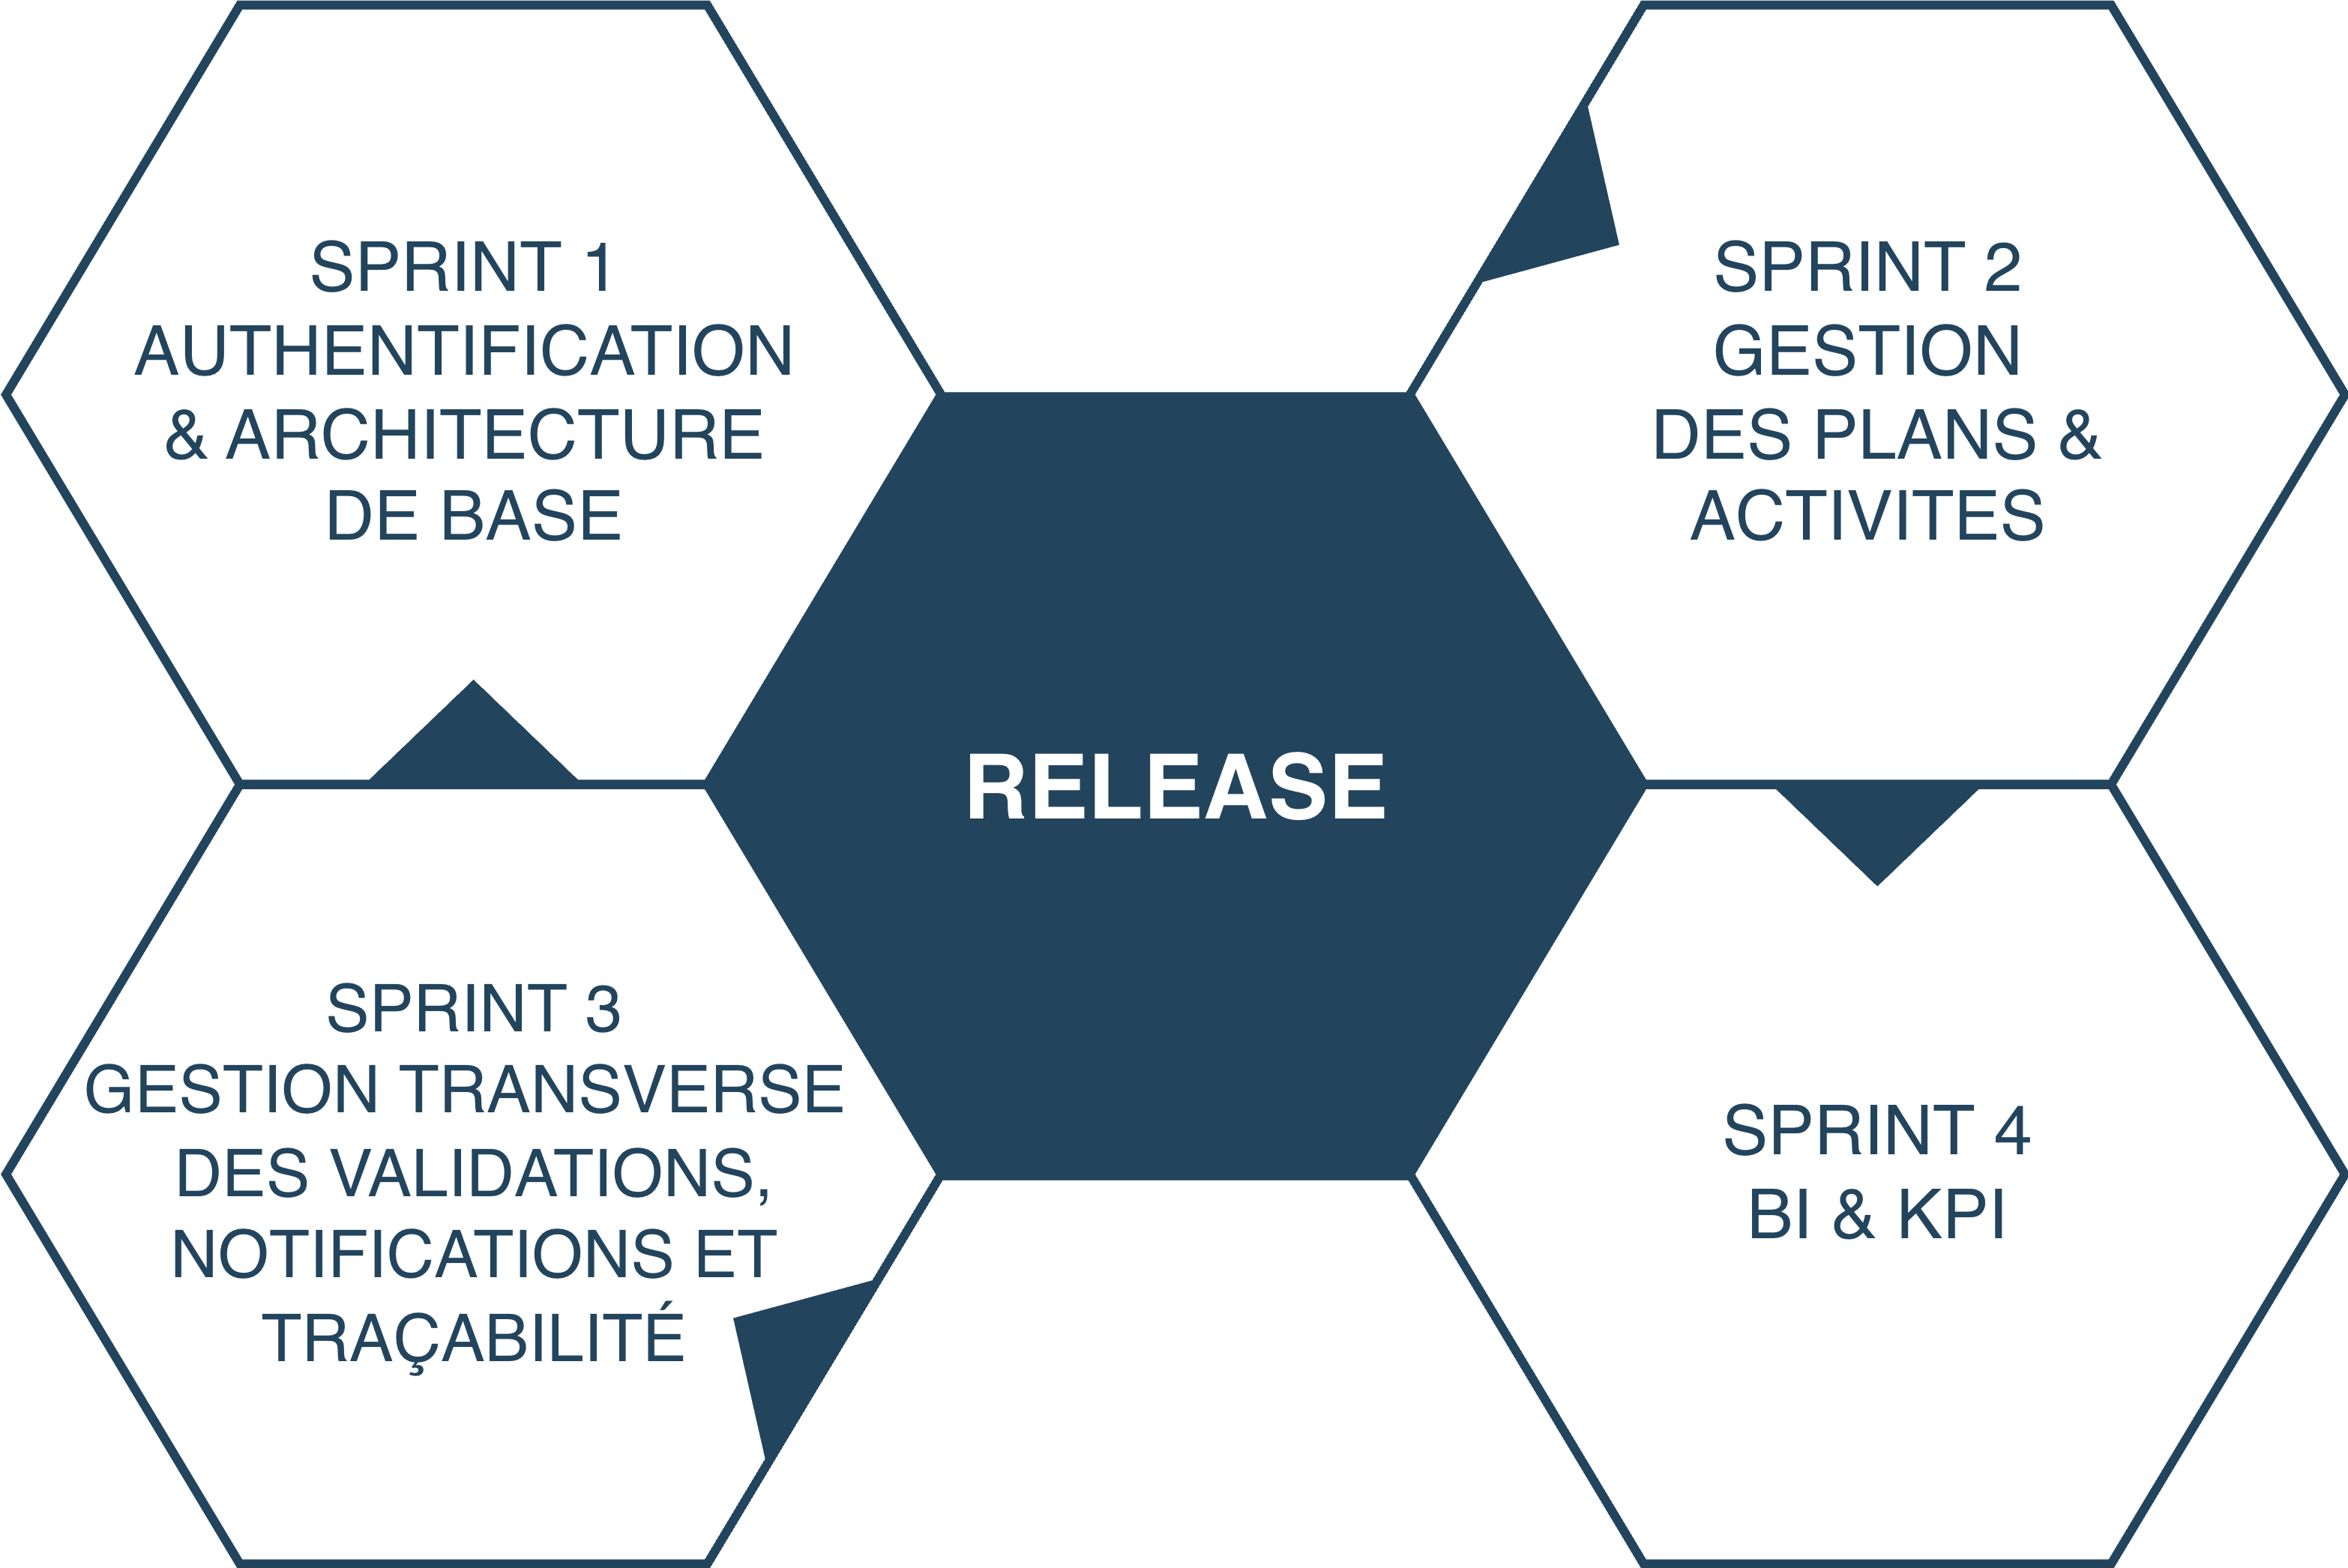
\includegraphics[width=0.9\linewidth]{figures/chapitre-02/Division-du-projet.png}
  \caption{Division du projet en sprints.}
  \label{fig:doc-ch2-division-projet}
\end{figure}

\begin{table}[H]
  \centering
  \small
  \caption{Méthode GIMSI adaptée dans un contexte Scrum.}
  \label{tab:ch02-gimsi-phases}
  \PFETableSetup
  % Tableau plus large que le bloc de texte : déborde de façon symétrique dans les marges.
  \makebox[\textwidth][c]{%
  \begingroup
  \renewcommand{\tabularxcolumn}[1]{>{\raggedright\arraybackslash}m{#1}}%
  \PFETableArrayStretch
  \arrayrulecolor{black}%
  \begin{tabularx}{\dimexpr\PFETableBlockWidth+2.8cm\relax}{%
    |>{\centering\arraybackslash}m{3.1cm}%
    |>{\centering\arraybackslash}m{0.55cm}%
    |>{\raggedright\arraybackslash}m{2.45cm}%
    |>{\raggedright\arraybackslash}X|}%
    \hline
    \tableHeaderStyle
    \tableHeaderCell{Phase} &
    \tableHeaderCell{N\textsuperscript{o}} &
    \tableHeaderCell{Étape} &
    \tableHeaderCell{Adaptation dans Scrum} \\
    \hline
    \multirow{2}{*}{\parbox{3.0cm}{\centering\bfseries Identification}} &
      \textbf{1} & Environnement de l’entreprise &
      Défini progressivement dans le Product Backlog. \\
    \cline{2-4}
    & \textbf{2} & Identification des acteurs &
      Réalisé via les User Stories et échanges avec les parties prenantes. \\
    \hline
    \multirow{5}{*}{\parbox{3.0cm}{\centering\bfseries Conception}} &
      \textbf{3} & Définition des objectifs &
      Affinés à chaque Sprint Planning. \\
    \cline{2-4}
    & \textbf{4} & Construction du tableau de bord &
      Conception itérative avec retour utilisateur. \\
    \cline{2-4}
    & \textbf{5} & Choix des indicateurs &
      KPI ajustés selon les besoins métiers évolutifs. \\
    \cline{2-4}
    & \textbf{6} & Collecte des informations &
      Données intégrées progressivement. \\
    \cline{2-4}
    & \textbf{7} & Système de tableaux de bord &
      Amélioration continue des tableaux de bord. \\
    \hline
    \multirow{2}{*}{\parbox{3.0cm}{\centering\bfseries Mise en œuvre}} &
      \textbf{8} & Choix des outils &
      Power BI retenu selon les besoins du projet. \\
    \cline{2-4}
    & \textbf{9} & Intégration &
      Réalisé par incréments à chaque sprint. \\
    \hline
    \parbox{3.0cm}{\centering\bfseries Suivi permanent} &
      \textbf{10} & Audit et amélioration &
      Amélioration continue via retours et itérations Scrum. \\
    \hline
  \end{tabularx}%
  \endgroup
  }%
\end{table}


\subsection{Planification des Sprints}

Après finalisation du \emph{product backlog}, nous avons estimé l’effort et le temps requis pour chaque élément et regroupé ceux-ci en phases de développement cohérentes. Le projet a été découpé en \textbf{quatre sprints}, chacun visant un ensemble de fonctionnalités du backlog avec une durée définie.

Le tableau~\ref{tab:ch02-planification-sprints} synthétise cette planification.

\begin{table}[H]
  \centering
  \small
  \caption{Planification du projet par sprints.}
  \label{tab:ch02-planification-sprints}
  \PFETableSetup
  \PFETableRowColors
  \PFETableArrayStretch
  \arrayrulecolor{black}
  \PFETableTabularXBegin
  \begin{tabularx}{\textwidth}{@{}>{\centering\arraybackslash}p{0.95cm}>{\raggedright\arraybackslash}p{2.35cm}>{\raggedright\arraybackslash}X>{\centering\arraybackslash}p{1.95cm}@{}}
    \hline
    \tableHeaderStyle
    \tableHeaderCell{N\textsuperscript{o}} &
    \tableHeaderCell{Nom du sprint} &
    \tableHeaderCell{Fonctionnalités couvertes} &
    \tableHeaderCell{Durée} \\
    \hline
    1 &
    Authentification \& Fondations &
    \begin{minipage}[t]{\linewidth}
      \begin{itemize}[leftmargin=*, itemsep=0.15ex, parsep=0pt, topsep=0.5pt, partopsep=0.5pt, label=\textbullet]
        \item Accès, rôles, cloisonnement (1)
        \item Fichiers (8)
        \item Référentiel entreprise/sites et documents (US\,1.4--1.5)
      \end{itemize}
    \end{minipage} &
    4 semaines \\
    \hline

    2 &
    Plans \& activités &
    \begin{minipage}[t]{\linewidth}
      \begin{itemize}[leftmargin=*, itemsep=0.15ex, parsep=0pt, topsep=0pt, partopsep=0pt, label=\textbullet]
        \item Plan annuel (2)
        \item Activités (3)
        \item Hors plan, indicateurs, pièces jointes, validation (5)
        \item Écarts planifié/réalisé et pilotage
      \end{itemize}
    \end{minipage} &
    4 semaines \\
    \hline
    3 &
    Workflow transverse &
    \begin{minipage}[t]{\linewidth}
      \begin{itemize}[leftmargin=*, itemsep=0.15ex, parsep=0pt, topsep=0pt, partopsep=0pt, label=\textbullet]
        \item Validation (2--3)
        \item Demandes de modification (4)
        \item Notifications (7)
        \item Chatbot (9)
        \item Tâches (11)
        \item Traçabilité (US\,2.7, 4.4)
      \end{itemize}
    \end{minipage} &
    4 semaines \\
    \hline
    4 &
    BI \& KPI &
    \begin{minipage}[t]{\linewidth}
      \begin{itemize}[leftmargin=*, itemsep=0.15ex, parsep=0pt, topsep=0pt, partopsep=0pt, label=\textbullet]
        \item Dashboards (5)
        \item Power BI (6)
        \item KPI et GIMSI (10)
      \end{itemize}
    \end{minipage} &
    3 semaines \\
    \hline
  \end{tabularx}
  \PFETableTabularXEnd
\end{table}



\subsection{Diagramme de classe générale}

La figure~\ref{fig:doc-ch2-3} illustre le diagramme de classe général de la solution. Le dictionnaire de données détaillant les attributs de ce schéma est fourni en annexe~B (tableau~\ref{tab:dictionnaire-donnees-classe}).

\clearpage
\newgeometry{margin=0pt}
\begin{landscape}
  \begingroup
  % Page dédiée au diagramme (sans footer/numéro/logo) + image au maximum de la page.
  \pagestyle{empty}
  \thispagestyle{empty}
  \captionsetup{aboveskip=2pt,belowskip=0pt,font=small}
  \begin{figure}[p]
    \thispagestyle{empty}
    \centering
    \includegraphics[
      width=1.3\paperwidth,
      height=\paperheight,
      keepaspectratio
    ]{figures/chapitre-02/diagramme-classe-general.png}
    \caption{Diagramme de classe général.}
    \label{fig:doc-ch2-3}
  \end{figure}
  \endgroup
\end{landscape}
\restoregeometry
\clearpage
\section{Architecture du système}

L’architecture de la plateforme est conçue pour orchestrer la création, la validation et l’exploitation des données CSR de manière sécurisée. Après authentification, le flux principal se divise en deux branches.
\par\addvspace{2ex}%

L’architecture repose sur une approche en couches permettant d’assurer une séparation claire des responsabilités et une meilleure maintenabilité du système. Elle s’organise autour de plusieurs niveaux : la couche de présentation, la couche d’authentification, la couche applicative, la couche de données opérationnelles et la couche décisionnelle.
\par\addvspace{2ex}%
Au niveau de la couche de présentation, l’utilisateur interagit avec une application web développée en Angular. L’accès aux fonctionnalités est sécurisé grâce à un mécanisme d’authentification basé sur des tokens JWT, géré par une API Flask dédiée.
\par\addvspace{2ex}%
La couche applicative est assurée par une API REST développée avec Flask, structurée en plusieurs modules métiers (plans, activités, workflow, documents, audit). Cette couche implémente la logique métier du système, notamment la validation des données, la gestion des droits d’accès et le pilotage des processus de workflow.
\par\addvspace{2ex}% 
Les données sont ensuite persistées dans une base de données MySQL via une couche ORM\footnote{ORM : \emph{Object-Relational Mapping} (mapping objet-relationnel). Il s’agit d’une approche de persistance qui met en correspondance les objets manipulés dans le code applicatif et les enregistrements d’une base relationnelle, afin de structurer les accès aux données et de limiter le SQL ad hoc~\cite{orm-wikipedia}. Dans ce projet, cette couche est assurée par SQLAlchemy et Flask-SQLAlchemy~\cite{sqlalchemy-docs}.}
, garantissant une abstraction efficace entre l’application et la base de données. Les fichiers et documents associés sont stockés dans un espace de stockage dédié.
\par\addvspace{2ex}%
Par ailleurs, la plateforme intègre un mécanisme de communication en temps réel via Socket.IO, permettant la diffusion instantanée des notifications et des mises à jour vers l’interface utilisateur.
\par\addvspace{2ex}%

Enfin, une couche décisionnelle vient compléter l’architecture. Les données issues de la base opérationnelle sont extraites, transformées et chargées via SSIS vers un Data Warehouse. Ce dernier est exploité à l’aide de SSMS pour la modélisation et l’analyse, puis connecté à Power BI pour la création de tableaux de bord interactifs et avancés. Cette séparation entre les systèmes transactionnels (OLTP) et analytiques (OLAP) permet d’optimiser les performances globales et de faciliter la prise de décision.

La figure~\ref{fig:doc-ch2-system-architecture} illustre l'architecture globale du système.

\begin{figure}[H]
  \centering
  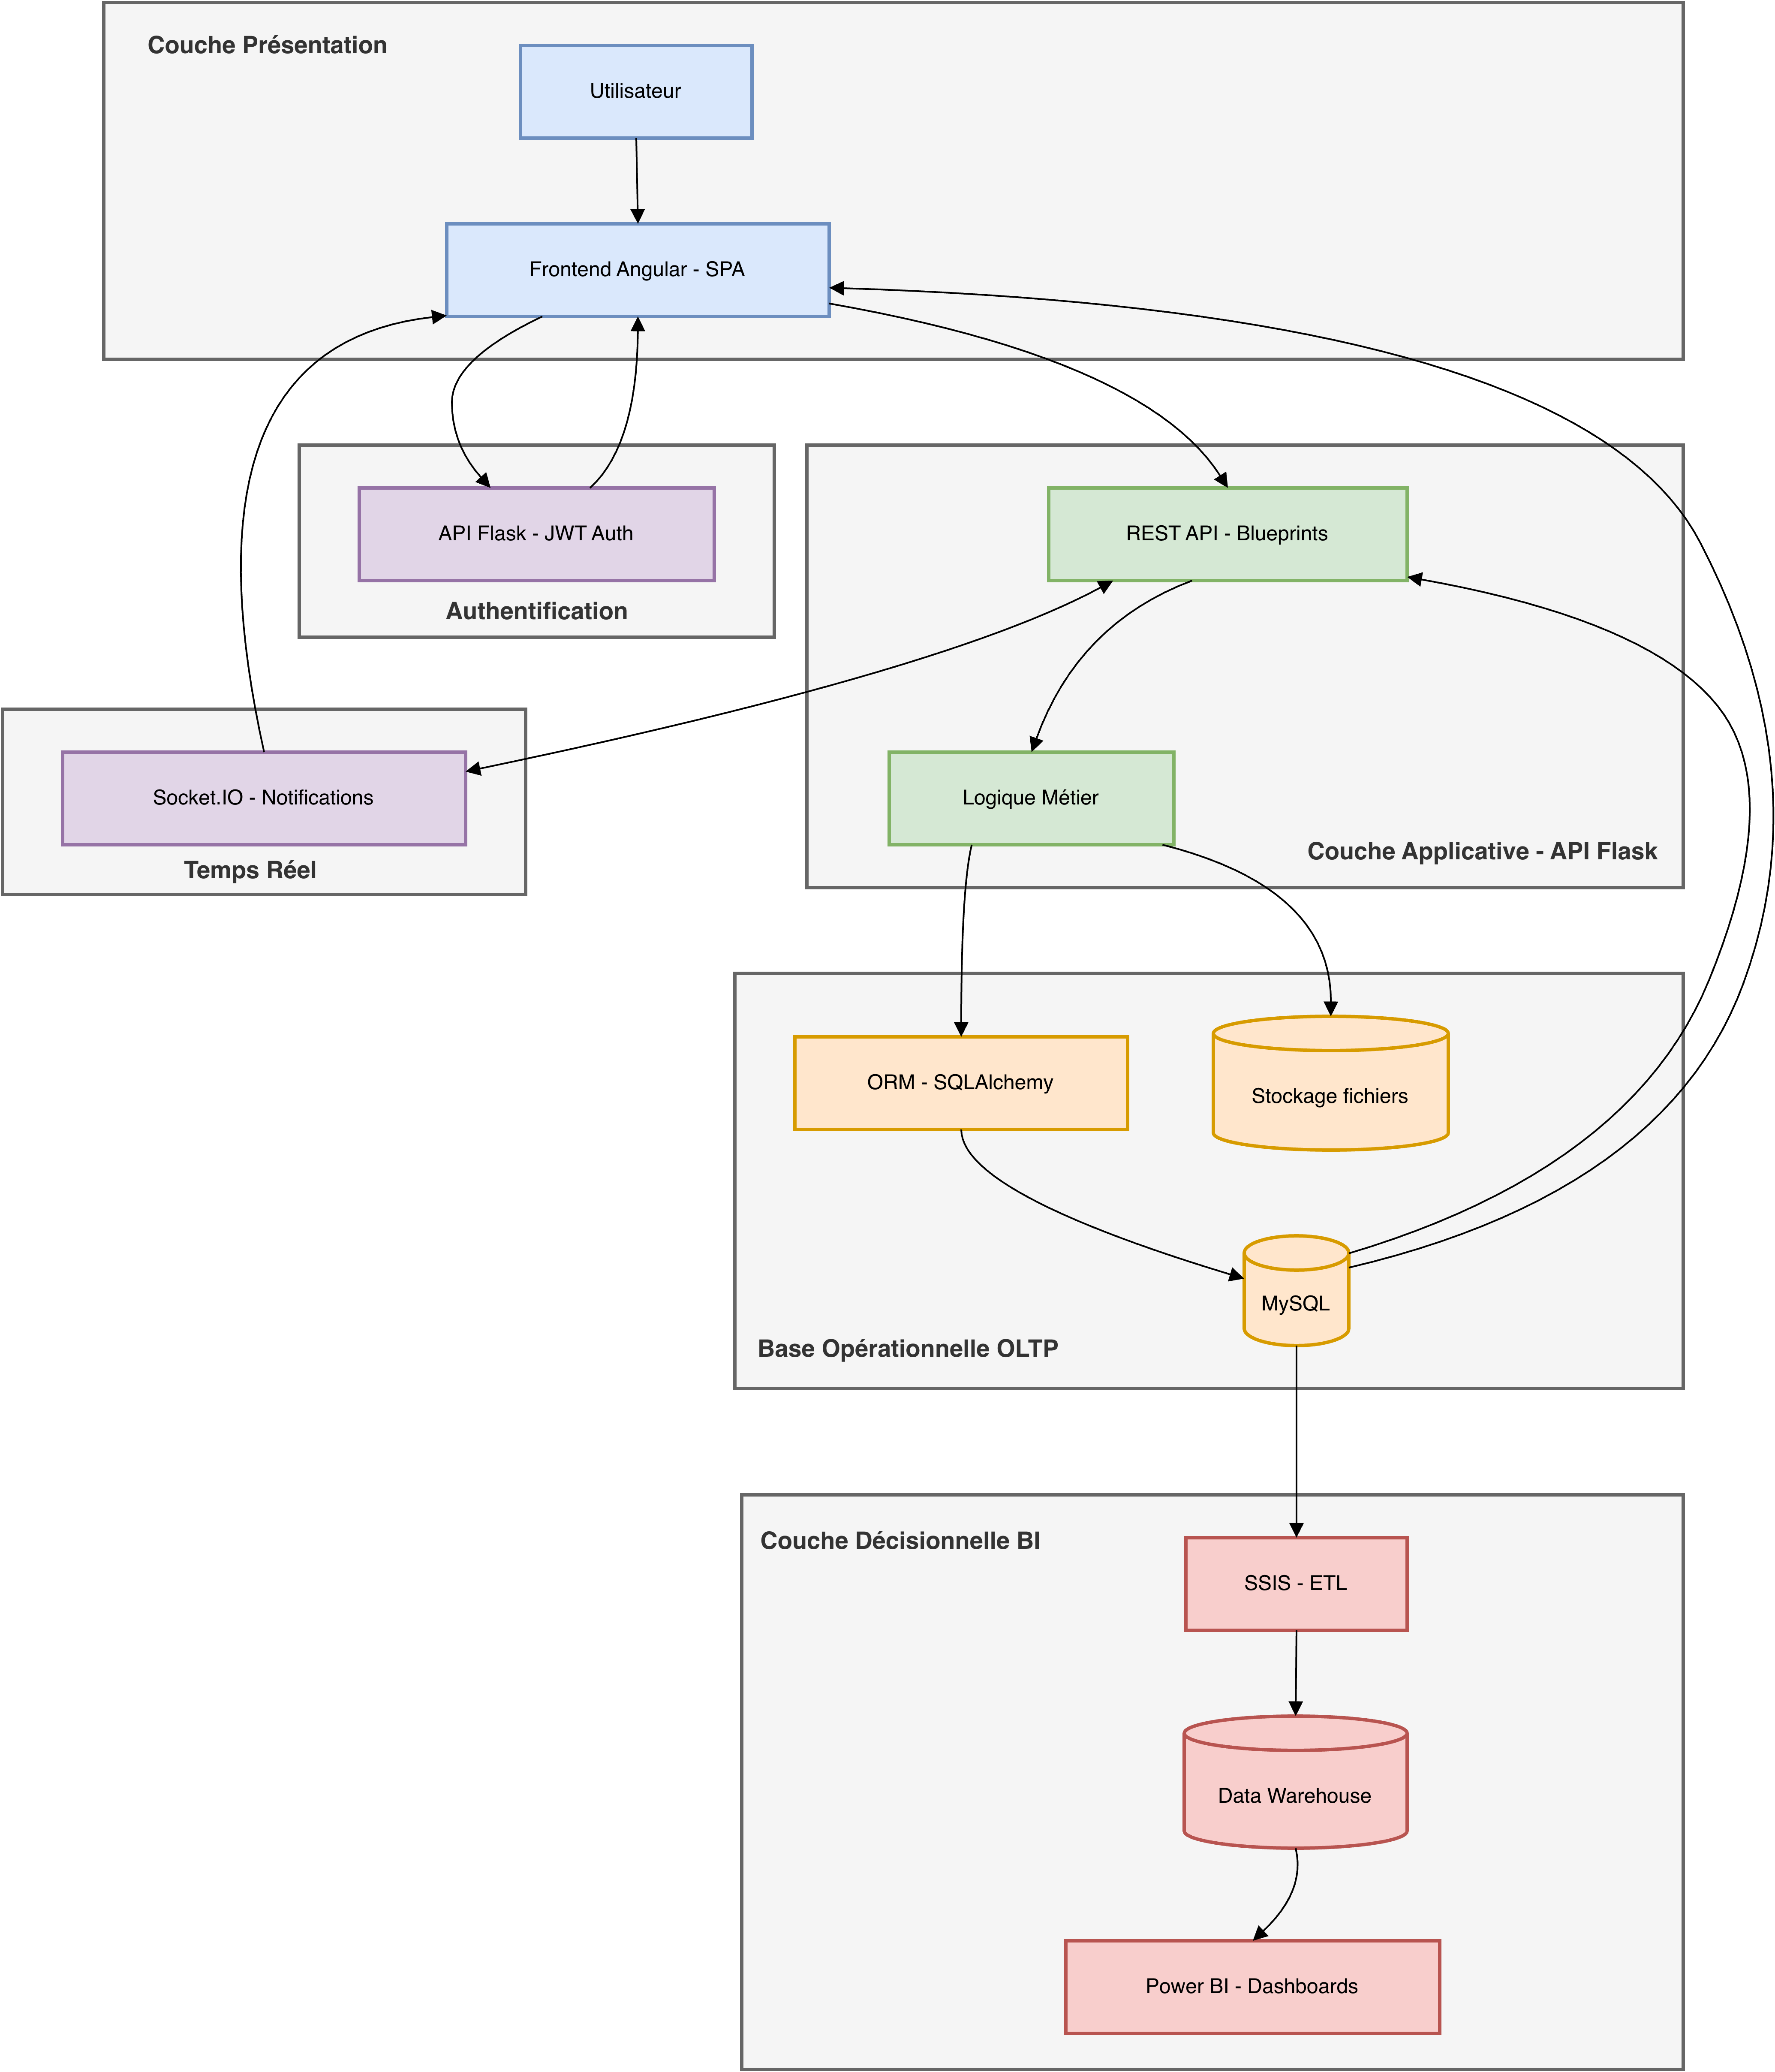
\includegraphics[width=\linewidth]{figures/chapitre-02/architecture-systeme-csr.png}
  \caption{Architecture globale du système.}
  \label{fig:doc-ch2-system-architecture}
\end{figure}
\footnote{SSIS : \emph{SQL Server Integration Services}. Il s’agit de la composante ETL (\emph{Extract, Transform, Load}) de SQL Server permettant de concevoir des flux d’intégration entre sources de données hétérogènes, de transformer et charger des données, puis d’orchestrer et de déployer ces traitements sous forme de packages~\cite{ssis-docs}.}
\footnote{SSMS : \emph{SQL Server Management Studio}. Il s’agit de l’outil graphique fourni par Microsoft pour administrer une instance SQL Server : exécution de requêtes T-SQL, gestion des bases et des schémas, configuration de la sécurité, sauvegardes et surveillance~\cite{ssms-docs}.}
\section{Choix des technologies}

Dans le cadre du développement de notre projet, nous avons retenu une pile technologique répondant aux exigences de \textbf{performance}, de \textbf{sécurité} (authentification, contrôle d’accès, cloisonnement par site) et de \textbf{scalabilité}. Chaque technologie a été choisie pour un rôle précis afin d’assurer une implémentation robuste et une maintenance aisée.


\subsection{Backend}

\vspace{0.35em}
\textbf{Python }\cite{python-docs} est un langage de programmation polyvalent, largement utilisé pour le développement web et l’intégration de services. 

La figure~\ref{fig:doc-ch2-tech-python-logo} présente le logo officiel de Python.
\begin{figure}[H]
  \centering
  
\includegraphics[height=1.8cm]{figures/chapitre-02/python.png}
  \caption[Logo de Python.]{Logo de Python.}
  \label{fig:doc-ch2-tech-python-logo}
\end{figure}

\vspace{0.35em}
\textbf{Flask }\cite{flask-docs} est un micro-framework Python \emph{open source} permettant de développer des applications web et des API REST de façon modulaire (blueprints, extensions). 

La figure~\ref{fig:doc-ch2-tech-flask-logo} présente le logo officiel de Flask.
\begin{figure}[H]
  \centering
  
\includegraphics[height=1.8cm]{figures/chapitre-02/flask.png}
  \caption[Logo de Flask.]{Logo de Flask.}
  \label{fig:doc-ch2-tech-flask-logo}
\end{figure}

\vspace{0.35em}
\textbf{MySQL}\cite{mysql-docs} est un système de gestion de base de données relationnelle fondé sur SQL, adapté au stockage structuré des entités métier et aux requêtes d’analyse.

La figure~\ref{fig:doc-ch2-tech-mysql-logo} présente le logo officiel de MySQL.
\begin{figure}[H]
  \centering
  
\includegraphics[height=1.8cm]{figures/chapitre-02/MySQL.png}
  \caption[Logo de MySQL.]{Logo de MySQL.}
  \label{fig:doc-ch2-tech-mysql-logo}
\end{figure}

\subsection{Frontend}

\vspace{0.2em}
\textbf{Angular }\cite{angular-docs} est un framework front-end basé sur des composants, proposant routage et injection de dépendances pour structurer une application web. 

La figure~\ref{fig:doc-ch2-tech-angular-logo} présente le logo officiel d’Angular.
\begin{figure}[H]
  \centering
  
\includegraphics[height=1.8cm]{figures/chapitre-02/angular.png}
  \caption[Logo d’Angular.]{Logo d’Angular.}
  \label{fig:doc-ch2-tech-angular-logo}
\end{figure}

\vspace{0.2em}
\textbf{TypeScript }\cite{typescript-docs} est un sur-ensemble typé de JavaScript, améliorant la robustesse du code (typage statique, outillage). 

La figure~\ref{fig:doc-ch2-tech-typescript-logo} présente le logo officiel de TypeScript.
\begin{figure}[H]
  \centering
  
\includegraphics[height=1.8cm]{figures/chapitre-02/TypeScript.png}
  \caption[Logo de TypeScript.]{Logo de TypeScript.}
  \label{fig:doc-ch2-tech-typescript-logo}
\end{figure}

\subsection{Interface utilisateur}

\vspace{0.2em}
\textbf{Tailwind CSS }\cite{tailwind-docs} est un framework utilitaire de styles permettant de composer rapidement des interfaces cohérentes. 

La figure~\ref{fig:doc-ch2-tech-tailwind-logo} présente le logo officiel de Tailwind CSS.
\begin{figure}[H]
  \centering
  
\includegraphics[height=1.8cm]{figures/chapitre-02/tailwind-css.png}
  \caption[Logo de Tailwind CSS.]{Logo de Tailwind CSS.}
  \label{fig:doc-ch2-tech-tailwind-logo}
\end{figure}

\vspace{0.2em}

\subsection{Communication temps réel}

\vspace{0.2em}
\textbf{Socket.IO }\cite{socketio-docs} est une bibliothèque de communication temps réel (événements) reposant sur WebSocket avec mécanismes de repli. 

La figure~\ref{fig:doc-ch2-tech-socketio-logo} présente le logo officiel de Socket.IO.
\begin{figure}[H]
  \centering
  
\includegraphics[height=1.8cm]{figures/chapitre-02/socket-io.png}
  \caption[Logo de Socket.IO.]{Logo de Socket.IO.}
  \label{fig:doc-ch2-tech-socketio-logo}
\end{figure}

\subsection{Outil de test}

\vspace{0.2em}
\textbf{Postman}\cite{postman-docs} est l’outil utilisé pour tester les API REST de la plateforme. Il permet de construire des requêtes, vérifier les réponses (succès/erreur) et valider les scénarios fonctionnels des endpoints backend.

La figure~\ref{fig:doc-ch2-tech-postman-logo} présente le logo de Postman.
\begin{figure}[H]
  \centering
  \IfFileExists{figures/chapitre-02/Postmam.png}{%
    
\includegraphics[height=2.cm]{figures/chapitre-02/Postmam.png}
  }{%
    \fbox{\parbox{4.6cm}{\centering\textit{Logo Postman à insérer}\\\texttt{figures/chapitre-02/Postmam.png}}}
  }
  \caption[Logo de Postman.]{Logo de Postman.}
  \label{fig:doc-ch2-tech-postman-logo}
\end{figure}

\section{Environnement et outils de développement}

Cette section décrit l’\textbf{environnement matériel} et l’\textbf{environnement logiciel} mobilisés pour concevoir, tester et documenter la plateforme.

\subsection{Environnement matériel}

Le développement a été réalisé sur \textbf{deux postes de travail}. 

Le tableau~\ref{tab:ch2-materiel} récapitule leurs caractéristiques principales.

\begin{table}[H]
  \centering
  \small
  \caption{Environnement matériel utilisé pour le développement.}
  \label{tab:ch2-materiel}
  \PFETableSetup
  \PFETableRowColors
  \PFETableArrayStretch
  \begin{tabular}{@{}>{\raggedright\arraybackslash}p{4.2cm}p{5.0cm}p{5.0cm}@{}}
    \tableHeaderStyle \tableHeaderCell{Élément} & \tableHeaderCell{MacBook Pro M1} & \tableHeaderCell{HP Vectus 15} \\
    Processeur (CPU) & M1 8 c\oe urs  & AMD Ryzen 5 5600H \\
    Carte graphique (GPU) & 8 c\oe urs (Apple GPU) & Nvidia GeForce GTX 1650 \\
    Neural Engine & 16 c\oe urs & 16 c\oe urs \\
    Mémoire vive & 8~Go & 24~Go RAM \\
    Stockage & SSD 256~Go & SSD 512~Go \\
    Système d’exploitation & macOS 26.3.1 (Tahoe) & Windows 11 (64 bits) \\
  \end{tabular}
\end{table}

\subsection{Environnement logiciel}

Notre projet s’appuie sur un ensemble d’outils logiciels adaptés aux phases de conception, de développement, de collaboration et de reporting. Chaque outil répond à un besoin précis afin d’assurer une mise en œuvre efficace et une documentation de qualité.

\subsection{Conception et architecture}

\vspace{0.2em}
\textbf{draw.io }\cite{diagrams-net-docs} est un outil de création de diagrammes (schémas d’architecture, diagrammes UML, organigrammes) avec export vers plusieurs formats. 

La figure~\ref{fig:doc-ch2-drawio-logo} présente le logo officiel de draw.io.

\begin{figure}[H]
  \centering
  
\includegraphics[height=1.4cm]{figures/chapitre-02/draw-io.png}
  \caption[Logo de draw.io.]{Logo de draw.io.}
  \label{fig:doc-ch2-drawio-logo}
\end{figure}

\subsection{Gestion de versions et collaboration}

\vspace{0.2em}
\textbf{Git }\cite{git-docs} est un système de contrôle de version distribué permettant de suivre l’historique, gérer des branches et faciliter le travail collaboratif. 

La figure~\ref{fig:doc-ch2-git-logo} montre le logo officiel de Git.
\begin{figure}[H]
  \centering
  
\includegraphics[height=1.4cm]{figures/chapitre-02/Git.png}
  \caption[Logo de Git.]{Logo de Git.}
  \label{fig:doc-ch2-git-logo}
\end{figure}

\vspace{0.2em}
\textbf{GitHub }\cite{github-docs} est une plateforme d’hébergement de dépôts Git offrant des fonctionnalités de collaboration (issues, pull requests, revue de code). 

La figure~\ref{fig:doc-ch2-github-logo} montre le logo officiel de GitHub.
\begin{figure}[H]
  \centering
  
\includegraphics[height=1.4cm]{figures/chapitre-02/github.png}
  \caption[Logo de GitHub.]{Logo de GitHub.}
  \label{fig:doc-ch2-github-logo}
\end{figure}

\vspace{0.2em}
\textbf{Monday.com }\cite{monday-docs} est un outil de gestion de projet et de travail collaboratif basé sur des tableaux visuels, facilitant l’organisation des tâches, le suivi de l’avancement et la coordination des équipes.

La figure~\ref{fig:doc-ch2-monday-logo} présente le logo officiel de Monday.com.
\begin{figure}[H]
  \centering
  
\includegraphics[width=8cm]{figures/chapitre-02/Monday_logo.svg.png}
  \caption[Logo de Monday.com.]{Logo de Monday.com.}
  \label{fig:doc-ch2-monday-logo}
\end{figure}

\subsection{Développement}

\vspace{0.2em}
\textbf{Visual Studio Code }\cite{vscode-docs} est un éditeur de code extensible et multiplateforme proposant notamment l’auto-complétion, le débogage et l’intégration Git. 

La figure~\ref{fig:doc-ch2-vscode-logo} présente le logo officiel de Visual Studio Code.
\begin{figure}[H]
  \centering
  
\includegraphics[height=3cm]{figures/chapitre-02/visual-studio-code.jpeg}
  \caption[Logo de Visual Studio Code.]{Logo de Visual Studio Code.}
  \label{fig:doc-ch2-vscode-logo}
\end{figure}

\vspace{0.2em}
\textbf{Microsoft Visual Studio } \cite{visualstudio-docs} est un environnement de développement intégré (IDE) permettant de concevoir, compiler, tester et déboguer des applications. 

La figure~\ref{fig:doc-ch2-visualstudio-logo} présente le logo officiel de Microsoft Visual Studio.
\begin{figure}[H]
  \centering
  
\includegraphics[height=1.4cm]{figures/chapitre-02/Microsoft-Visual-Studio.png}
  \caption[Logo de Microsoft Visual Studio.]{Logo de Microsoft Visual Studio.}
  \label{fig:doc-ch2-visualstudio-logo}
\end{figure}

\vspace{0.2em}
\textbf{Microsoft SQL Server } \cite{sqlserver-docs} est un système de gestion de base de données relationnelle (SGBDR) développé par Microsoft, destiné au stockage et à l’analyse de données. 

La figure~\ref{fig:doc-ch2-sqlserver-logo} présente le logo officiel de Microsoft SQL Server.
\begin{figure}[H]
  \centering
  
\includegraphics[height=1.4cm]{figures/chapitre-02/sql-serveur.png}
  \caption[Logo de Microsoft SQL Server.]{Logo de Microsoft SQL Server.}
  \label{fig:doc-ch2-sqlserver-logo}
\end{figure}

\vspace{0.2em}
\textbf{Mapping objet-relationnel (ORM)} \cite{orm-wikipedia} désigne une approche de persistance qui établit une correspondance entre les objets manipulés dans le code applicatif et les tables (ou vues) d’une base relationnelle, afin de structurer les accès aux données et de réduire le SQL répétitif. Dans le backend de la plateforme CSR, cette couche est assurée par \textbf{SQLAlchemy} \cite{sqlalchemy-docs} (avec Flask-SQLAlchemy comme pont vers l’API Flask). 

La figure~\ref{fig:doc-ch2-sqlalchemy-logo} présente le logo de SQLAlchemy.
\begin{figure}[H]
  \centering
  
\includegraphics[height=1.4cm]{figures/chapitre-02/sqlalchemy.png}
  \caption[Logo de SQLAlchemy (ORM et accès SQL).]{Logo de SQLAlchemy (ORM et accès SQL).}
  \label{fig:doc-ch2-sqlalchemy-logo}
\end{figure}

\vspace{0.2em}
\textbf{XAMPP }\cite{xampp-docs} est une distribution regroupant un serveur web (Apache) et des composants associés (dont MySQL/MariaDB et PHP), utilisée pour mettre en place rapidement un environnement serveur local. 

La figure~\ref{fig:doc-ch2-xampp-logo} montre le logo officiel de XAMPP.
\begin{figure}[H]
  \centering
  
\includegraphics[height=1.4cm]{figures/chapitre-02/Xampp.png}
  \caption[Logo de XAMPP.]{Logo de XAMPP.}
  \label{fig:doc-ch2-xampp-logo}
\end{figure}

\subsection{Reporting et documentation}

\vspace{0.2em}
\textbf{Power BI }\cite{powerbi-docs} est une plateforme de \emph{business intelligence} permettant de créer des rapports et tableaux de bord interactifs. 

La figure~\ref{fig:doc-ch2-powerbi-logo} montre le logo officiel de Power BI.
\begin{figure}[H]
  \centering
  
\includegraphics[height=1.8cm]{figures/chapitre-02/power-bi.png}
  \caption[Logo de Power BI.]{Logo de Power BI.}
  \label{fig:doc-ch2-powerbi-logo}
\end{figure}

\vspace{0.2em}
\textbf{LaTeX } \cite{latex-docs} est un système de composition de documents basé sur \TeX, permettant de produire des documents structurés avec une typographie stable. 

La figure~\ref{fig:doc-ch2-latex-logo} présente le logo officiel de \LaTeX.
\begin{figure}[H]
  \centering
  
\includegraphics[height=1.8cm]{figures/chapitre-02/LaTeX_project_logo_bird.png}
  \caption[Logo de \LaTeX.]{Logo de \LaTeX.}
  \label{fig:doc-ch2-latex-logo}
\end{figure}

\section{Conclusion}

Ce chapitre a posé les bases du projet : exigences fonctionnelles, démarche Scrum, formalisation du \emph{product backlog} et des \emph{user stories}, planification et chronologie des sprints, puis architecture et choix technologiques. Les environnements matériel et logiciel mobilisés pour concevoir la plateforme CSR ont également été décrits. Les chapitres suivants présentent successivement les quatre sprints retenus — \emph{Authentification \& Fondations}, \emph{Plans \& activités}, \emph{Workflow transverse}, \emph{BI \& KPI} — et leur mise en œuvre.
